
% to choose your degree
% please un-comment just one of the following
\documentclass[bsc,frontabs,twoside,singlespacing,parskip,deptreport]{infthesis}     % for BSc, BEng etc.
% \documentclass[minf,frontabs,twoside,singlespacing,parskip,deptreport]{infthesis}  % for MInf

\usepackage[utf8]{inputenc}
\usepackage{epigraph}
\usepackage{graphicx} %Added by Songbo

% Flexible Qoute

\usepackage{epigraph,varwidth}

\renewcommand{\epigraphsize}{\small}
\setlength{\epigraphwidth}{0.6\textwidth}
\renewcommand{\textflush}{flushright}
\renewcommand{\sourceflush}{flushright}
% A useful addition
\newcommand{\epitextfont}{\itshape}
\newcommand{\episourcefont}{\scshape}

\makeatletter
\newsavebox{\epi@textbox}
\newsavebox{\epi@sourcebox}
\newlength\epi@finalwidth
\renewcommand{\epigraph}[2]{%
  \vspace{\beforeepigraphskip}
  {\epigraphsize\begin{\epigraphflush}
   \epi@finalwidth=\z@
   \sbox\epi@textbox{%
     \varwidth{\epigraphwidth}
     \begin{\textflush}\epitextfont#1\end{\textflush}
     \endvarwidth
   }%
   \epi@finalwidth=\wd\epi@textbox
   \sbox\epi@sourcebox{%
     \varwidth{\epigraphwidth}
     \begin{\sourceflush}\episourcefont#2\end{\sourceflush}%
     \endvarwidth
   }%
   \ifdim\wd\epi@sourcebox>\epi@finalwidth 
     \epi@finalwidth=\wd\epi@sourcebox
   \fi
   \leavevmode\vbox{
     \hb@xt@\epi@finalwidth{\hfil\box\epi@textbox}
     \vskip1.75ex
     \hrule height \epigraphrule
     \vskip.75ex
     \hb@xt@\epi@finalwidth{\hfil\box\epi@sourcebox}
   }%
   \end{\epigraphflush}
   \vspace{\afterepigraphskip}}}
\makeatother

% End Flexiable Qoute


\begin{document}

\title{Building Coherent Open-domain Dialogue Systems Using Neural Networks}

\author{Songbo Hu}

% to choose your course
% please un-comment just one of the following
\course{Artificial Intelligence and Computer Science}
%\course{Artificial Intelligence and Software Engineering}
%\course{Artificial Intelligence and Mathematics}
%\course{Artificial Intelligence and Psychology }   
%\course{Artificial Intelligence with Psychology }   
%\course{Linguistics and Artificial Intelligence}    
%\course{Computer Science}
%\course{Software Engineering}
%\course{Computer Science and Electronics}    
%\course{Electronics and Software Engineering}    
%\course{Computer Science and Management Science}    
%\course{Computer Science and Mathematics}
%\course{Computer Science and Physics}  
%\course{Computer Science and Statistics}    

% to choose your report type
% please un-comment just one of the following
%\project{Undergraduate Dissertation} % CS&E, E&SE, AI&L
%\project{Undergraduate Thesis} % AI%Psy
\project{4th Year Project Report}

\date{\today}

\abstract{
Add abstract later.
}

\maketitle

\section*{Acknowledgements}
Acknowledgements go here. 

\tableofcontents

%\pagenumbering{arabic}

\chapter{Introduction}

\epigraph{When was Alan Turing born? \\
Alan Turing was born on Sunday 13 June 1912. \\
Where was he born? \\
Alan Turing was born in Warrington Lodge. \\
Who is his father? \\
Julius Mathison Turing is Alan Turing's father.\\
When was he born? \\
Julius Mathison Turing was born 9 November 1873. \\
Where? \\
You're at Edinburgh, Scotland.
}{\textit{Songbo and Siri 2020}}

A dialogue system is a conversational agent that can converse with humans in natural language. It can help us solve many tedious tasks effectively or bring entertainment value to our daily life. Recent advances in dialogue systems (such as virtual assistants) enable us to engage in natural conversational interactions with computers. It substantially increases the accessibility of state of the art technologies to people with diverse backgrounds. And for those with impairments, it could transform their daily living into a journey toward capability instead of disability.

Since Alan Turing published his landmark work in 1950\cite{turing1950computing}, the intelligence level of a machine is described as how well the machine is able to fool a human into believing that it, the machine, is a human based on its text responses. If the human evaluator cannot tell the difference between the machine from a human, the machine is said to have passed the Turing test, which signifies a high level of intelligence of an AI. It has been the goal for the development of dialogue systems for decades and there are various attempts have been proposed to pass the Turing test. Recently, advances in neural network based language models enable us to learn entire dialogue models directly from conversational data. But we are still far from our goal. Most of the previous systems have failed to model the longer prior context of the conversation adequately, thereby creating a situation where extended dialogues rapidly become incoherent and unnatural sounding, with repetition being a key problem. Like I mentioned above, Siri fails to model anaphoras and elided constructions and produces repetitive and incoherent responses. It is a problem which need to be adequately solved before our agents could look forward to passing the Turing test.

In this section, we will briefly review the recent development of dialogue systems. Specifically, we will discuss two types of dialogue systems: the chit-chat dialogue system and goal-oriented dialogue system, particularly current statistical spoken dialogue system (hereafter SDS). We will discuss their architectures, pros and cons, and their main limitations to achieve coherent open-domain conversations. The majority of this thesis is about how to create an environment for neural models to learn linguistic patterns within coherent extended dialogues and how to integrate these models into the existing dialogue systems. It constitutes a first step towards modelling coherent open-domain conversations and will potentially enable the existing dialogue systems utilising useful linguistic information and produce coherent responses.

\section {A Brief Review of Existing Dialogue Systems}

\subsection{The Chit-chat Dialogue System}

The chit-chat dialogue systems are usually called chatbots. These systems are designed and implemented to carry extended conversations with the goal of mimicking the unstructured conversations or ‘chats’ characteristic of informal human-human interaction. They are mainly aiming to provide entertainment value. Existing chatbots majorly fall into the following subcategories: the rule-based systems, the corpus-based systems, as will be discussed in order below.

\subsubsection*{The rule-based systems}

Instead of letting machines learning the conversation strategy from human behaviours, we could ask humans to encode these human intelligence directly as rules and ask machines to interpret them. Dialogue agents could use these rules to generate dialogue utterances effectively. Normally, a message input will be processed by a set of carefully pre-defined rules e.g., a key-word look-up dictionary, if-else conditions, or more sophisticated machine learning classifiers. After rule conditions are evaluated, relevant actions will be executed, such as outputting an utterance in storage, manipulating the input message or selecting some related historical contexts.

\begin{figure}[h]
    \centering
    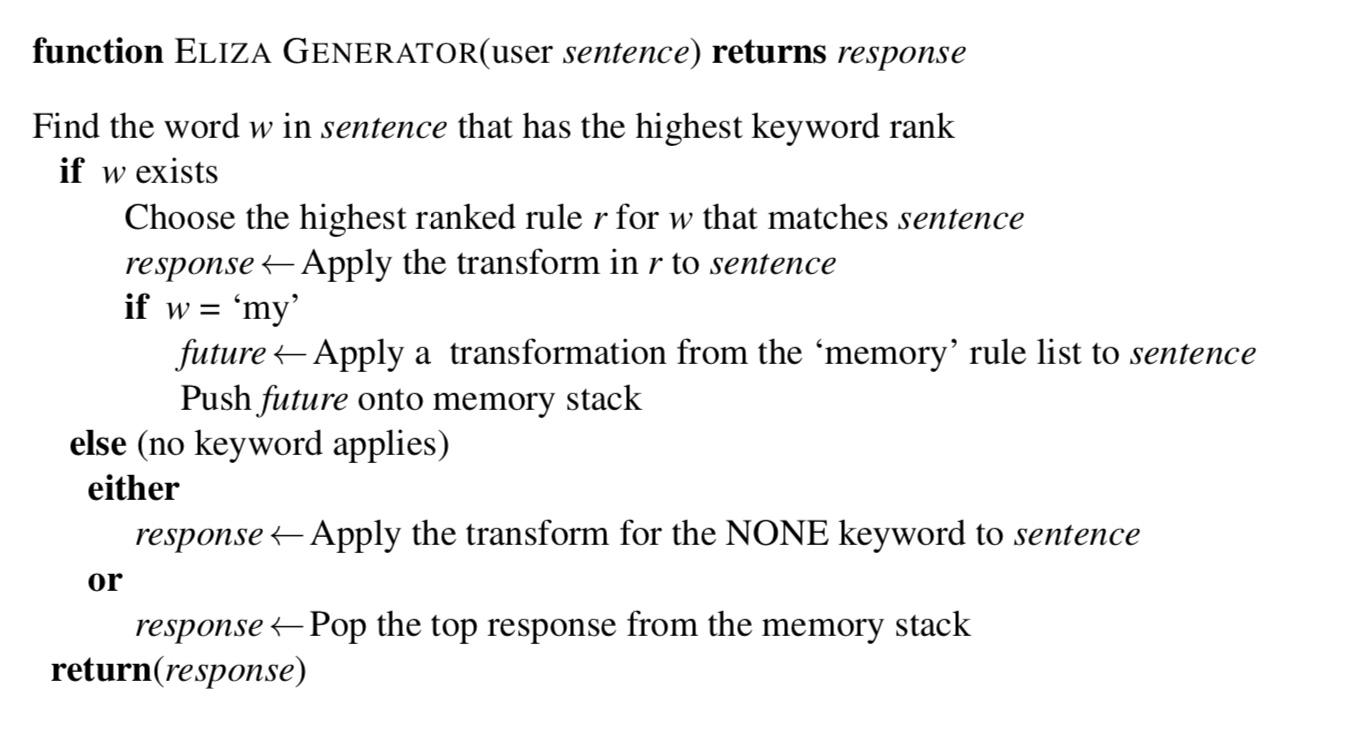
\includegraphics[width=0.9\textwidth]{elizarule.jpeg}
    \caption{A simplified sketch of the ELIZA algorithm.}
    \label{fig:elizarule}
\end{figure}

One of the epoch-making rule-based dialogue systems in history is ELIZA\cite{weizenbaum1966eliza}. ELIZA operates by first searching a keyword existing in the input text from a real human based on a hand-crafted keyword dictionary. If a keyword is found, a rule is applied to manipulate and transform the user’s original input and forwarded back to the user. Otherwise, ELIZA responded either with a generic response or copying one sentence from the dialogue history. There are many extensions of ELIZA, for example, PARRY\cite{parkinson1977conversational} and ALICE\cite{wallace1995artificial}. PARRY,, which simulated a patient with schizophrenia, relies on global variables to keep track of the emotional state, as opposed to ELIZA where responses are generated only based on the previous sentence. Artificial Intelligence Markup Language(AIML), which is the basis of ALICE, provides an effect tool to write sophisticated conversations logic in a machine-readable format.

ELIZA-style systems are recognized as an important milestone in developing modern dialogue systems. Even nowadays, with the rapid development of large fancy neural network architecture and increasing number of conversational corpora, these rule-based dialogue systems could always be a very strong baseline. On the other hand, their drawbacks are obvious: Rule-based systems predominantly rely on the set of pre-defined rules and these rules have to be carefully designed and implemented. Building a sophisticated rule-based system is very expensive because the number of these rules skyrockets. Rule-based systems do not have the ability to understand human languages, nor do they know how to generate meaningful natural language utterances. Consequently, they are very brittle and only able to conduct very superficial conversations.

\subsubsection*{The corpus-based systems}

Coding conversations logic manually is astronomically expensive and infeasible for many applications. Corpus-based dialogue system could potentially mitigate this issue by mining conversations of human-human conversations, or sometimes mining the human responses from human-machine conversations, instead of using hand-built rules. These data-driven approaches are becoming increasingly popular due to the increasing computing power and the creation of large scale conversational data-set. 

There are two common architectures for such system:  information retrieval (IR), and machine learned sequence transduction. Due to the limitation that IR-based chatbots can only mirror training data, it is often to treat response generation as a machine translation task which transduces from the user’s prior turn to the system’s turn. This method offers the promise of scalability and language-independence, together with the capacity to implicitly learn semantic and syntactic relations between pairs, and to capture contextual dependencies in a way not possible with IR-based approaches.

\begin{figure}[h]
    \centering
    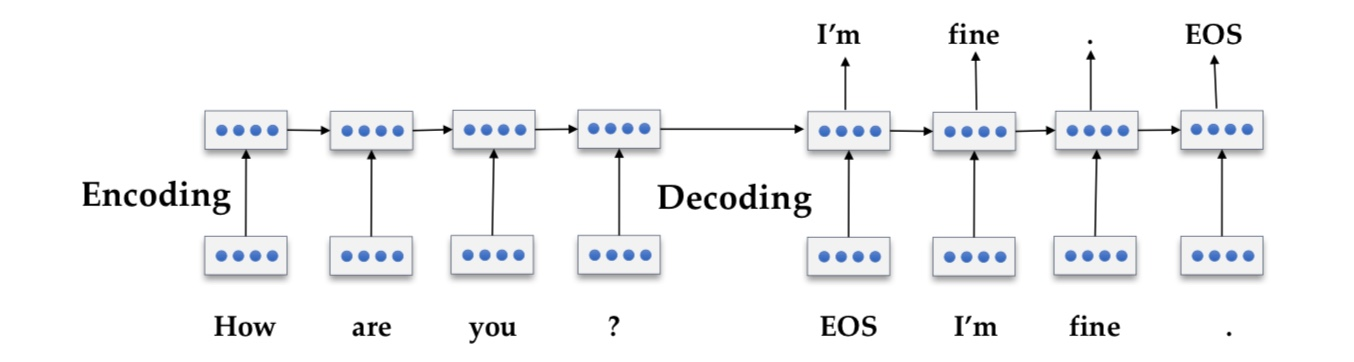
\includegraphics[width=0.9\textwidth]{seq2seq.jpeg}
    \caption{A sequence to sequence model for neural response generation.\cite{jurafsky2019speech}}
    \label{fig:seq2seq}
\end{figure}

This idea was firstly developed by Ritter et al\cite{ritter2011data}. (cited in Jurafsky and Martin\cite{jurafsky2019speech}) using phrase-based machine translation to translate a user turn to a system response. In 2015, transduction models for response generation were modelled instead using encoder-decoder (seq2seq) models\cite{shang2015neural,strub2017end,sordoni2015neural}. However, the simple seq2seq generation architecture is unable to model the prior context of the conversation. Serban et al\cite{serban2016building} suggests a hierarchical (HRED) model that summarizes information over multiple prior turns. This model consists of two recurrent neural networks (RNNs) stacked on top of each other: one is a sentence-level RNN which encodes each utterance into a fixed length vector, while a conversation-level RNN takes as input each utterance vector and outputs a vector that summarizes the conversation so far. The vector is mapped back to text using a recurrent decoder. This gives a way for the previous information to be passed to future turns as hidden states\cite{lowe2017training}.

\begin{figure}[h]
    \centering
    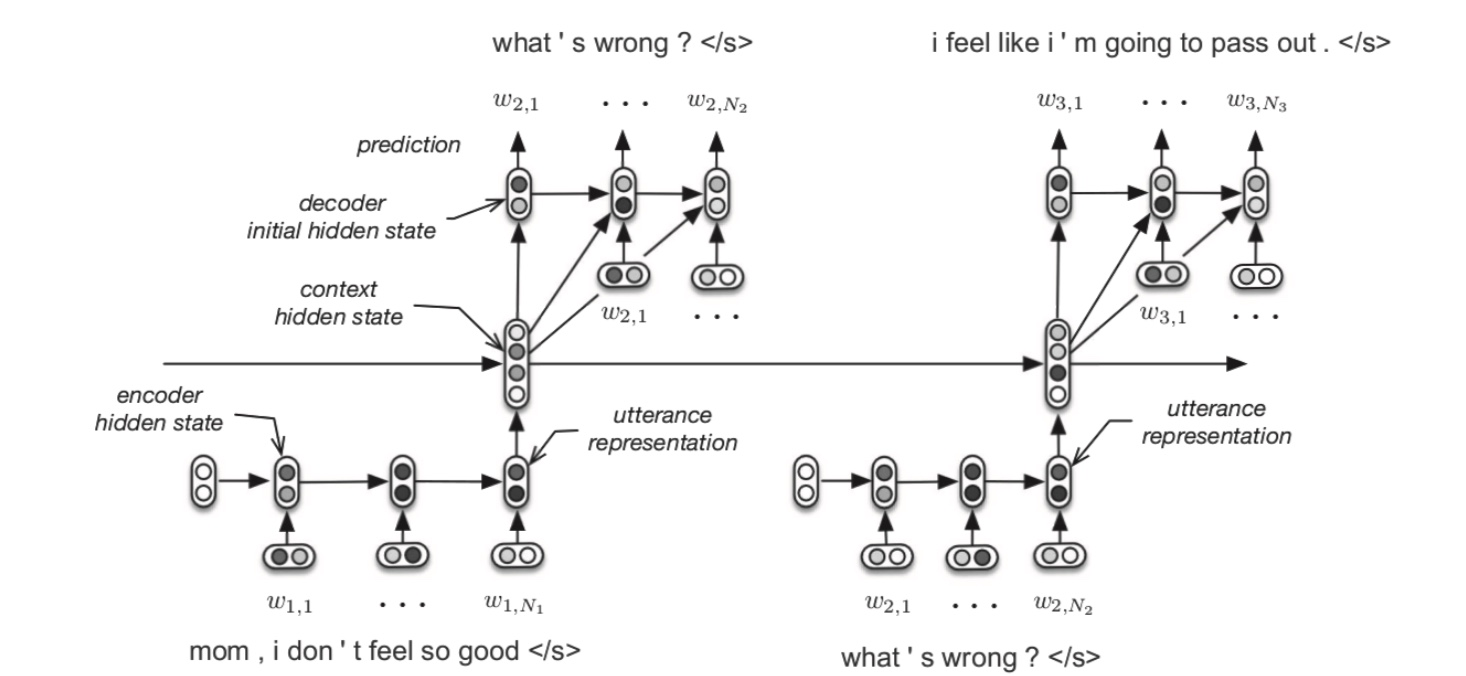
\includegraphics[width=0.9\textwidth]{HERD.jpeg}
    \caption{The computational graph of the HRED architecture for a dialogue composed of three turns.}
    \label{fig:HERD}
\end{figure}

However, even if one has access to an enormous dataset for training, there is still a significant proportion of unseen dialogue states. Techniques, such as smoothing, can only help to a limited extent, because of the radical extent to which data is sparse. Consequently, generating responses using end-to-end methods tends to generate generic, uninformative and non-coherent replies (e.g., generating ``I don’t know." regardless of the context). In addition, encoder-decoder response generators focus on generating single responses, instead of forming a coherent continuous conversation\cite{jurafsky2019speech}. Humans could easily notice these unnatural and mechanical responses (e.g. the Siri conversation above). Techniques, such as Reinforcement learning (RL) and adversarial networks, will be introduce in Chapter 2 to address this issue\cite{li2017adversarial}\cite{li2016deep}.

\subsection{The Goal-oriented Dialogue system}

 Goal-oriented Dialogue systems are sometimes also called task-based dialogue systems, in which they use conversation with users to help complete tasks like making an airplane reservation, booking a hotel or buying a product. Famous examples of such agents are digital assistants (Siri, Alexa, Google Home, Cortana, et.). With the power of cloud computing and internet of things technologies, these conversations AIs are changing our daily life and developing a 10 billion pounds worth industry (add citation). Here, I would like to introduce the architectures of existing statistical spoken dialogue systems (hereafter SDSs) and their main challenges to perform coherent conversations in an open domain. 

\begin{figure}[h]
    \centering
    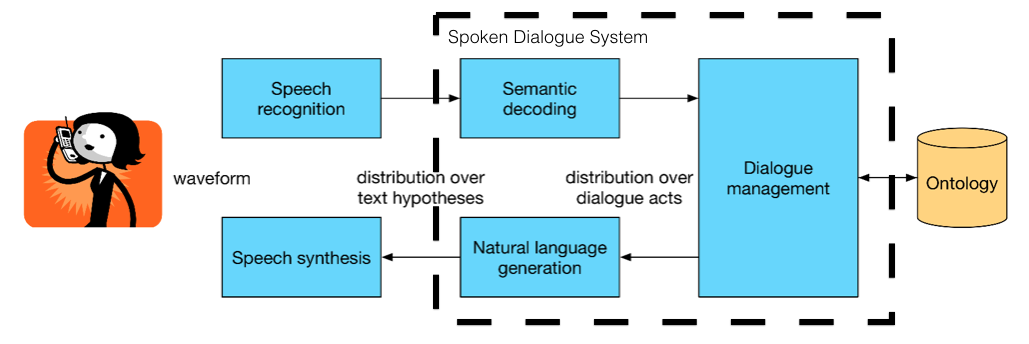
\includegraphics[width=0.80\textwidth]{sds.png}
    \caption{Architecture of a Spoken Dialogue System.\cite{gasic}}
    \label{fig:sds}
\end{figure}

Current SDSs have three key components which are shown as Figure \ref{fig:sds}. Semantics decoder decodes the meaning in utterances into dialogue acts which describe the current intention of the user, for example, confirm(food=Korean). Then, dialogue manager, which usually consists of a belief tracker and a policy network, will keep track of the belief states and produce a dialogue act as the response. Dialogue manager treats dialogue generation as a partially observable Markov decision processes (POMDPs)\cite{williams2007partially,young2013pomdp,young2010hidden} which explicitly models the uncertainty natural of human conversations with Bayesian methods. Such framework provides robustness against the errors created by speech recognizers operating in noisy environments. Later a semantic encoder (natural language generator) will map this act back into natural language.

However, keeping track of the belief states under such a framework presents a tough challenge. Exact model representation is infeasible due to the limitation of computational complexity\cite{young2013pomdp}. Carefully constructed approximation and additional independent assumption are needed. For example, if we are willing to find an expensive 5-star hotel in the city center, in order to make the inference practical, we have to assume that there is no relation between a hotel to be expensive and it is a 5-star hotel. It is clearly not true. In addition, as shown in Figure\ref{fig:sds}, pre-defined ontology is needed in order to keep track of the dialogue state. This makes the existing dialogue system infeasible to perform conversations in an open-domain. One research direction would be build a SDS which can support a natural conversation about any topic within a wide coverage Knowledge Graph (KG). This forms the definition of an open-domain spoken dialogue system (Add citation)\cite{http://mi.eng.cam.ac.uk/research/dialogue/EPSRCProj/stories/desc.html}.


\section {Thesis Outline}

In this dissertation, we mainly address problems involved in the chit-chat system and the interactive QA system. First, we explore how to build an engaging chit-chat style dialogue system that is able to conduct interesting, meaningful, coherent, consistent, and long-term conversation with humans. More specially, for the chit-chat system, we (a) use mutual information to avoid dull and generic responses (Li et al., 2016a,c, 2017c); (b) address user consistency issues to avoid inconsistent responses from the same user (Li et al., 2016b); (c) develop reinforcement learning methods to foster the long-term success of conversations (Li et al., 2016d); and (d) use adversarial learning methods to generate machine responses that are indistinguishable from human-generated responses (Li et al., 2017d);
Second, we explore how a bot can best improve itself through the online interactions with humans that makes a chatbot system trully INTERACTIVE. We develop interactive di- alogue systems for factoid question-answering: (a) we design an environment that provides the agent the ability to ask humans questions and to learn when and what to ask (Li et al., 2017b); (b) we train a conversation agent through interaction with humans in an online fashion, where a bot improves through communicating with humans and learning from the mistakes that it makes (Li et al., 2017a).
CHAPTER1. INTRODUCTION 10
We start off by providing background knowledge on SEQ2SEQ models, memory net- work models and policy gradient reinforcement learning models in Chapter 2. The afore- mentioned four problems for the chit-chat style dialogue generation systems will be de- tailed in Chapters 3,4,5,6, and the two issues with the interactive QA system will be de- tailed in Chapters 7 and 8. We conclude this dissertation and discuss future avenue for chatbot development in Chapter 9.







\chapter{Background}

\section{Modelling Dialogues}
\subsection{N-gram Models}
\subsection{Recurrent Neural Networks and its Variations}
RNN
Long Short Term Memory
\subsection{Attention Mechanism}
\subsection{Self-Attentional Model}
\subsection{Pre-Trained Language Embedding}

\section{Machine Learning Paradigms for Dialogue Modelling}
\subsection{Supervised Learning}
\subsection{Unsupervised Learning}
\subsection{Reinforcement Learning}
Talk about Deep Reinforcement Learning for Dialogue Generation\cite{li2016deep} and Adversarial learning for neural dialogue generation \cite{li2017adversarial}.


\section{Corpora for Training Dialogue Models}
\subsection{Chit-chat Dataset}
Ubuntu
Twitter
...
\subsection{Goal-Oriented Dialogue Dataset}
\subsubsection*{Task-Oriented}
\subsubsection*{Visual Question Answering}
\subsubsection*{Corpus Grounded on Other Types of Knowledge}

\section{Dialogue Model Evaluation}
\subsection{Intrinsic Evaluation}
Perplexity
BLEU Score
...
Talk about their limitation.
\subsection{Extrinsic Evaluation}
Evaluation on Downstream tasks.
Question Answering Tasks. Precision Recall F1
Goal Oriented.

\subsection{Human Evaluation}
Best but expensive.



\chapter{Extended Dialogues Grounded on Knowledge Graph: A Corpus}
\section{Corpus Design}
I will talk about the motivation of this corpus. I will talk about what does this dataset looks like and how it is annotated.

\section{comparison with Related Work}



\section{Implementation}
\subsubsection*{Sampling from Knowledge Graph}

\subsubsection*{Web-interface for Data Collection}

\subsubsection*{Tools for Annotating the Dataset}

\section{Data Collection Procedure}
\subsubsection*{Advertising the Experiment}
\subsubsection*{Scheduling the Experiment}
\subsubsection*{Payment Method}

\chapter{Statistical Analysis}

Size of the corpus.
Average length of the dialogue and sentences.
Work token ratio.
Statistic about how many proroun, how many anaphoras and elided constructions per turn.
Statistic about question types.

Comparison of the above spastics when there is a topic shift or not.

Comparison of the above spastics when the domain is familiar or not.

\chapter{Modelling Coherent Dialogues Using Neural Networks}
I will write proposed neural model here.

\chapter{Towards Building Coherent Open-domain Dialogue Systems}
I will write how to integrate the neural with existing dialogue system. 

\chapter{Discussion}

\chapter{Conclusion and Future Work}



% use the following and \cite{} as above if you use BibTeX
% otherwise generate bibtem entries
\bibliographystyle{plain}
\bibliography{mybibfile}

\end{document}